\beginsong{Schon so lang}[wuw={A. Campbell, deutscher Text: Hannes Wader}, bo={41}, pfii={182}, gruen={197}, biest={516}, siru={32}, index={Bin auf meinem Weg}]

\beginverse
\endverse
\centering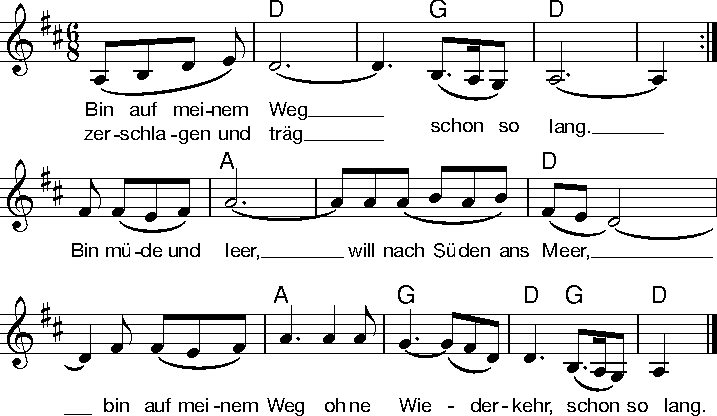
\includegraphics[width=1\textwidth]{Noten/Lied080a.pdf}	

\beginverse
Seh die Kriege in \[D]Not, \[G]schon so \[D]lang, Ruinen und Tod, \[G]schon so \[D]lang,
seh die Tränen, die \[A]Wut, seh die Wunden, das \[D]Blut,
erwürgt und ver\[A]fault, was \[G]stark war und \[D]gut, \[G]schon so \[D]lang.
\endverse

\beginverse
Seh' die Welt oft im ^Traum, ^schon so ^lang, als Pilzwolkenbaum, ^schon so ^lang.
Euch, ihr Herren der ^Welt, eure Lügen, den ^Mord,
an Millionen, die ^glauben an ^euer ^Wort, ^schon zu ^lang.
\endverse

\beginverse
Nicht nur Greuel ge^scheh'n, ^schon so ^lang. Hab' die Liebe geseh'n, ^schon so ^lang.
Seh' die Hoffnung, den ^Mut, seh den Glauben, die ^Glut
und was sich in Ge^sichtern von ^Kindern ^tut, ^schon so ^lang.
\endverse

\beginverse
Bin auf meinem ^Weg, ^schon so ^lang, zerschlagen und träg, ^schon so ^lang.
Bin müde und ^leer, will nach Süden ans ^Meer,
bin auf meinem ^Weg ohne ^Wieder^kehr, ^schon so ^lang.
\endverse

\endsong

\begin{intersong}
\ifthenelse{\boolean{pics}}{
    \ThisTileWallPaper{\paperwidth + 5mm}{\paperheight + 5mm}{Bilder/LenaRausch_Weg.png}
}{}
\end{intersong}
